\documentclass[main.tex]{subfiles}

\pagestyle{fancy}
%\fancyhf{}
\rhead{Assignment 2 - Boundary Layer Transition}
\lhead{AE4130 | 4738942}
\renewcommand{\headrulewidth}{0.1pt}

\begin{document}
\section{Problem Statement}
The aim of this assignment is to understand and clearly elucidate the influence of the amplification factor(n-factor) on the behavior of the boundary layer and the airfoil characteristics. This is done through the help of the program XFOIL. Changing the n-factor for several incident angles($\alpha$), different results for $C_p$ and $C_F$ are obtained. The drag polars for 2 different airfoils, namely the NACA 2715 and the much more cambered NACA 4412 is used to understand the simulation of roughness and its influence on lowering the $C_D$.
\section{Theory and Procedure}
In most aircraft flow boundary conditions, the flow across the wing is usually turbulent with very high Reynolds numbers. This is studied through a turbulent flow, wherein the flow stays attached throughout the wing (atleast for this case). At lower Reynolds number, i.e. for laminar flow, there is a strong adverse pressure gradient along the surface on the airfoil. At a certain location, this laminar boundary layer (flow still attached to airfoil) separates and transitions into a turbulent state. This is the transition location. The region between the separated laminar flow and turbulent flow is the laminar separation bubble. The presence of such a bubble increases the boundary layer and thus increases the drag of the airfoil. This complex phenomenon of laminar flow, transition, turbulent flow and then reattachment is a non-linear phenomenon and has been studied extensively.\\
\indent For the prediction of transition point especially, the $e^n$ method (linear stability theory) developed by \textit{Prof.J.L. van Ingen\cite{van1956suggested}} is well suited. The main problem being that the value of n is initially an unknown quantity. n is typically a function of the free stream turbulence level. Experiments by \textit{Smith et.al.\cite{smith1956transition}} and independently by \textit{van Ingen} showed that transition occurs at values of $n=9$. XFOIL also makes use of this $e^n$ method and uses a default value of $n = 9$. n is a representation of the ambient turbulence level, which can vary depending on other boundary conditions. For flows with greater turbulent intensity this method may not give agreeable results, hence creating the need to understand the effect of n-factor. To understand its influence, drag polars, $C_L$ vs $\alpha$ plots and other boundary layer characteristics are plotted and discussed in the upcoming sections.
\subsection{Airfoil Selection}
The conversion of student registration number to a NACA designated airfoil yielded the following;
\begin{table}[b]
\begin{center}
\begin{tabular}{ c c c } 
 \hline
 \rowcolor{lightgray}
 Student Number & N & NACA Airfoil \\
 \hline
 4738942 & 15 & 2715  \\ 
 \hline
\end{tabular}
\label{table1}
 \caption{Calculation of 4-series airfoil shape}
\end{center}
\end{table}
For the second part of the assignment NACA 4412(non-symmetrical airfoil) was chosen, since its slightly more cambered than NACA 2715. The length of the transition bubble can be better visualized and quantitatively understood. The 2 airfoils shapes are shown in Figure \ref{Fig1}.\vspace*{-0.5em}
\begin{figure}[h]
\centering
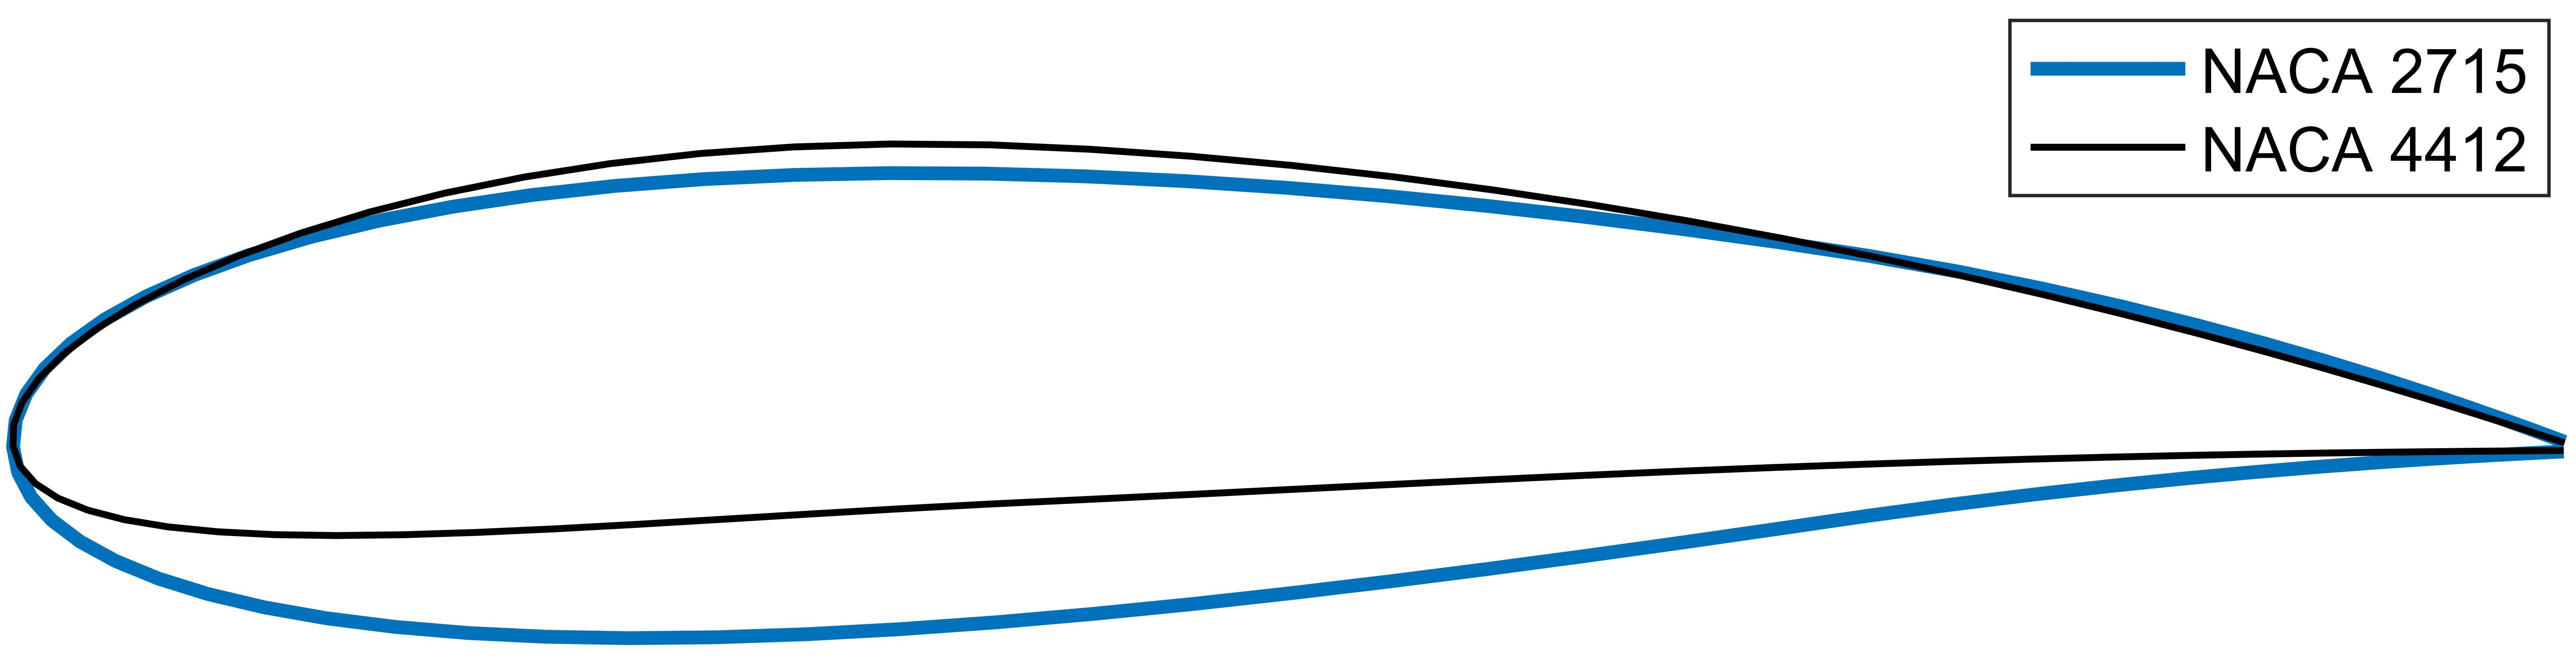
\includegraphics[scale=0.06]{./Images/Ass2/Airfoil_Comparison} 
\caption{Airfoil shape comparison between NACA 2715 and NACA 4412}\vspace*{-0.9em}
\label{Fig1}
\end{figure}
\section{Results and Conclusion}\vspace*{-0.9em}
\subsection{3.1	Part I - Effect of n factor on NACA 2715}
\vspace*{-2em}
\begin{figure}[h!]
    \centering
    \subfloat[Drag polar for NACA 2715]{
        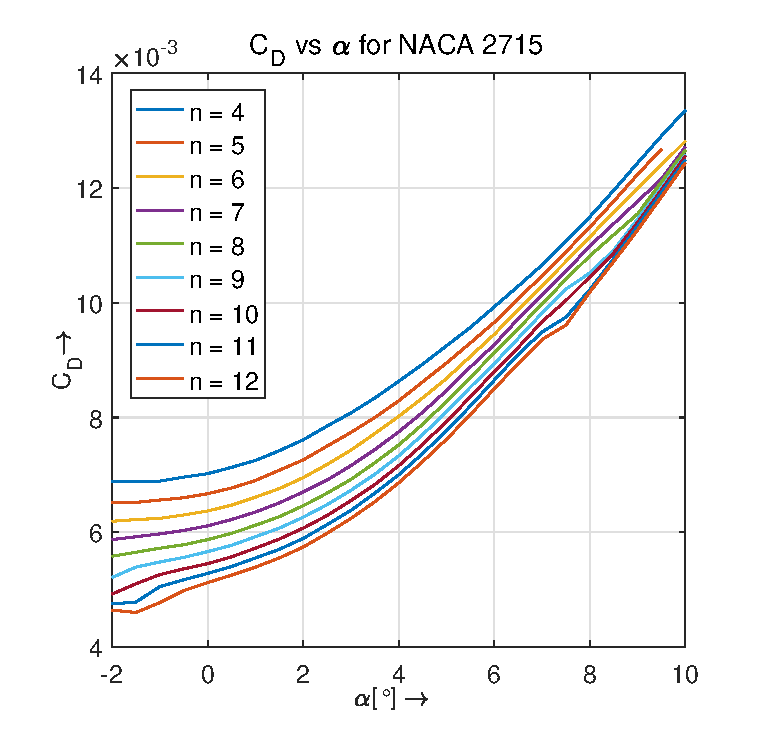
\includegraphics[width=0.5\textwidth] {./Images/Ass2/CDvsAlpha}
        \label{fig2a} } \hspace*{-1.2em}
    \subfloat[Lift polar for NACA 2715]{
        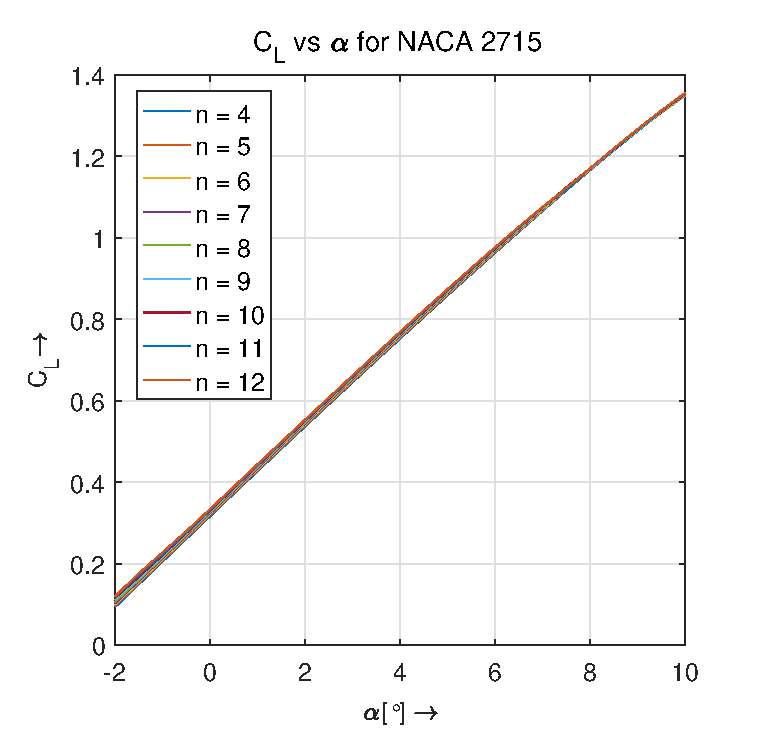
\includegraphics[width=0.5\textwidth] {./Images/Ass2/CLvsAlpha}
        \label{fig2b} } \\\vspace*{-0.8em}
         \subfloat[Lift vs drag polar for NACA 2715]{
        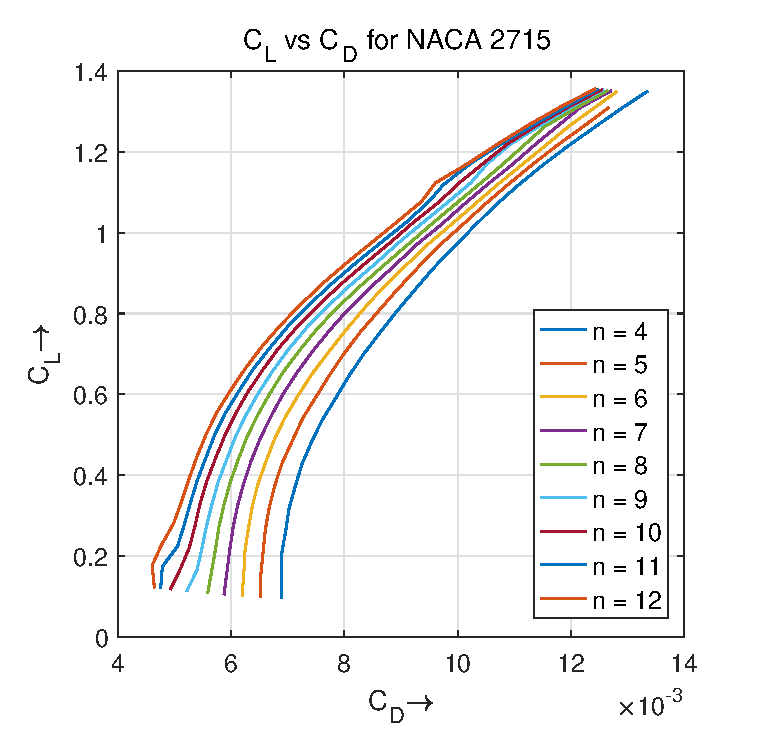
\includegraphics[width=0.5\textwidth] {./Images/Ass2/DragPolar}
        \label{fig2c} } \hspace*{-1.2em}
    \subfloat[$C_F$ vs $x/c$ for NACA 2715]{
        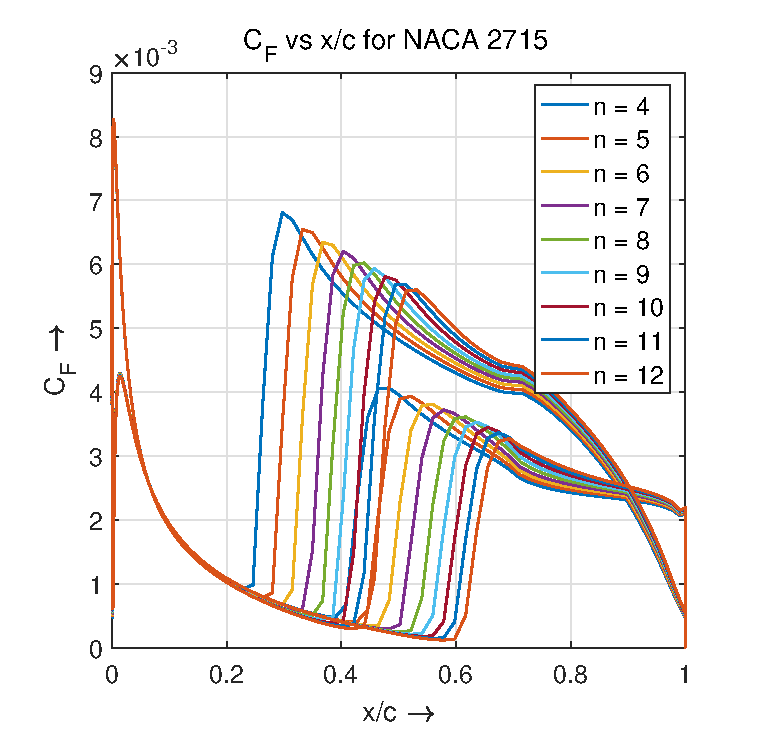
\includegraphics[width=0.5\textwidth] {./Images/Ass2/CFvsX}
        \label{fig2d} } \\\vspace*{-0.5em}
    \caption{Lift and Drag polar for $\alpha$  -2$^{\circ}$ to 10$^{\circ}$ for n 4 to 12}
    \label{fig2}
\end{figure}
\pagebreak
\\To understand the effect of n-factor, the XFOIL analysis program was used to generate the lift and drag polar between $-2^{\circ}$ and $10^{\circ}$ angle of attack at a $R_e$ of $3\times10^{6}$. Figure \ref{fig2a} shows the $C_D$ vs $\alpha$ plot for varying n values. High values of n resulting in a lower drag coefficient. This is expected, since the n value is indication of the level of disturbance in the flow stream. A higher value of n corresponds to a more laminar flow around the airfoil. To understand this, lets consider a constant $\alpha$ of $2^{\circ}$ in Figure \ref{fig2a}. As we move from $n=12$ to $n=4$, the drag coefficient increases by about 30\%. Figure \ref{fig2d} helps in supporting this reasoning as well. For lower n factors, the transition point starts to develop early on, i.e. towards the leading edge, resulting in a slightly longer separation bubble(seen in Figure \ref{fig2d}). 
\\\indent In other words, the area enclosed by the shear stress plot for $n=4$ is larger. This should mean that the net drag for the airfoil is larger. This is exactly what is show in the drag polars of Figure \ref{fig2}. Based on this observation we can further conclude that the length of the separation is an indication of the increase in drag. More the length more the drag. Literature also states that if the bubble bursts, besides an increase in drag a significant loss in lift can also be expected. But such bubble bursting phenomenon is not seen in these studies since XFOIL cannot predict this phenomenon. 
\\\indent At higher incidence angles, the gradient in $C_D$ is steeper. This is obvious, since at higher $\alpha$, the transition point further moves towards the leading edge due to the destabilizing pressure gradient. Also, at these high incidence angles the induced drag contributes more than the skin friction drag. This effect is being elucidated in Part II of this assignment.\vspace*{-0.9em}
\subsection{Part 2 - Simulation of Roughness (Forced Transition)}
\\\indent The new non-symmetrical airfoil, NACA 4412 is analyzed here for understanding the effect of n factor, as well as understanding how for a fixed lift coefficient, the drag coefficient is influenced by changing location of forced transition. To clearly understand the effect of laminar separations, a slightly lower $R_e$ of $5\times10^{5}$ is used.\vspace*{-1.7em}
\begin{figure}[h!]
    \centering
    \subfloat[Pressure distribution for NACA 4412]{
        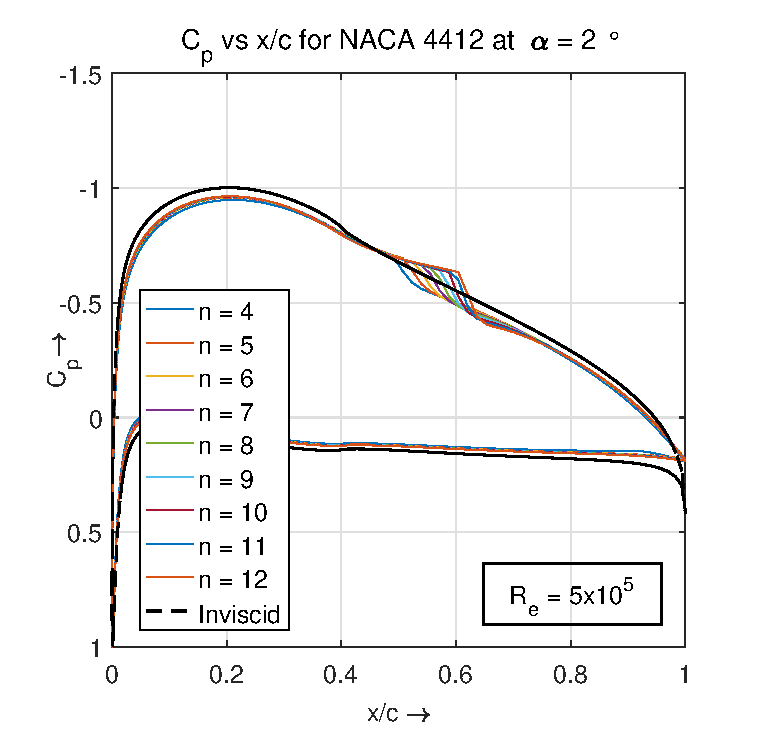
\includegraphics[width=0.5\textwidth] {./Images/Ass2/Cp_X_NACA4412}
        \label{fig3a} } \hspace*{-1.2em}
    \subfloat[Wall shear stress distribution for NACA 4412]{
        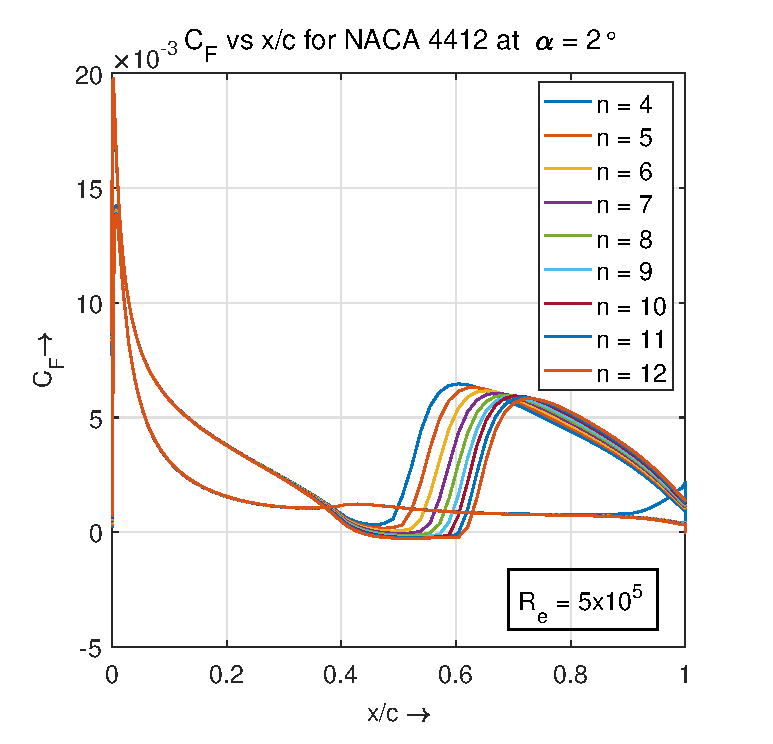
\includegraphics[width=0.5\textwidth] {./Images/Ass2/Cf_X_NACA4412}
        \label{fig3b} }\vspace*{-0.5em}
    \caption{$C_p$ and $C_F$ variations over NACA 4412}
    \label{fig3}
\end{figure}
\\\indent Figure \ref{fig3a} shows the pressure distribution for laminar flow over a cambered airfoil. The length of the separation bubble is characterized from the separation point to the reattachment point as mentioned in the work of \textit{Lee et al, 2006\cite{chen2008design}}. In Figure \ref{fig3a}, the point where the pressure gradient begins to plateau is the point where the separation begins. Assuming the bubble does not burst, the point of reattachment occurs where the $C_p$ curve continues to follow the normal trendline. Keeping this in mind, we can also visualize from Figure \ref{fig3a} that the longest separation bubble is obtained for the lowest n factor. This is a similar behavior as seen in Part I, lower n factor leading to larger drag coefficients. The wall shear stress variations in Figure \ref{fig3b} also have a very similar trend as seen in Part I. The wall shear stress have been plotted as a function of skin friction coefficient($C_F$). From both the figures it is very clear that the laminar separation occurs at $x/c\approx 0.5$ since the wall shear stress increases drastically and the recirculation zone has a continuously increasing shear stress. The increase in $C_F$ is expected due to formation of a turbulent recirculation region.\vspace*{-0.7em}
\begin{figure}[h!]
\centering
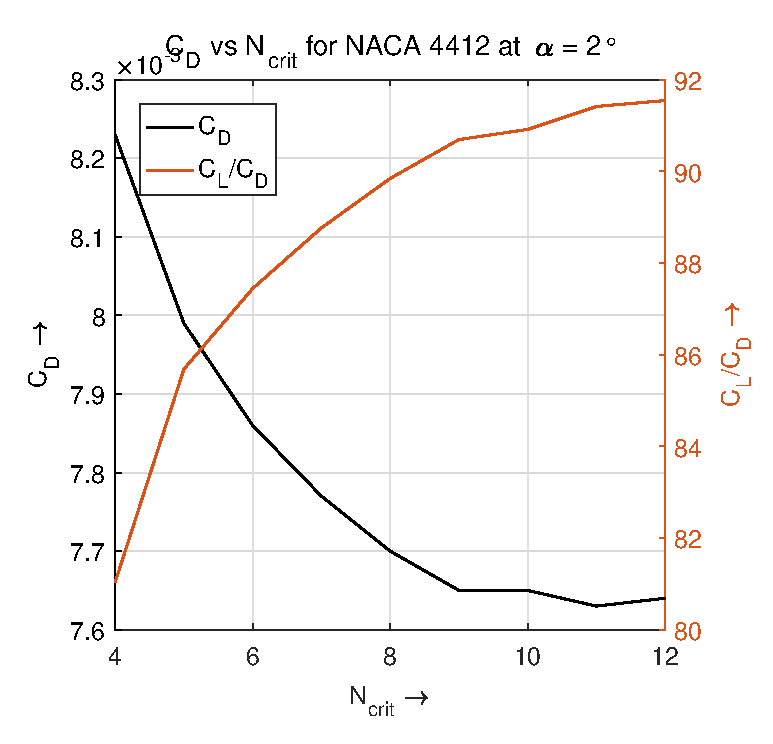
\includegraphics[width=0.5\textwidth]{./Images/Ass2/CdvsNcrit_NACA4412} 
\caption{$C_D$ vs $N_{crit}$ for NACA 4412}
\label{Fig4}
\end{figure}\vspace*{-0.7em}
\\\indent For the non-symmetrical airfoil NACA 4412, the $C_D$ vs $N_{crit}$ plot has been shown in Figure \ref{Fig4}. This decrease in $C_D$ agrees with our previous observations on the effect of n factor and further corroborates the fact that increasing n-factor leads to drag reduction.
\\\indent To understand the effect of forced transition on drag coefficient, the following boundary conditions in Table\ref{table2} were used in XFOIL.
\begin{table}[h!]
\begin{center}
\begin{tabu} to 0.5\textwidth {X[c] X[c]} 
 \hline
 \rowcolor{lightgray}
 Physical Quantity & Value \\
 \hline
 $R_e$ & $5\times10^{5}$  \\ 
 \hline
 $C_L$ & $0.3$  \\ 
 \hline
 $N_{crit}$ & $0.9$  \\ 
 \hline
 $\alpha$ & $2^{\circ}$  \\ 
 \hline
\end{tabu}
\caption{BCs for roughness simulation}\vspace*{-0.5em}
\label{table2}
\end{center}
\end{table}
\\\indent For a fixed $C_L$ value of $0.3$ the transition point of laminar separation is artificially controlled and set to values ranging between $0.05$ to $0.8$ of $x/c4$. For the current airfoil, the natural transition take place at $\approx80$\% of chord. Figure \ref{Fig5} shows the results of this study. A critical observation is that it is beneficial to have the laminar separation as late as possible(towards the aft of the airfoil), hence decreasing the drag as much as possible, but not beyond the natural transition point. For higher incidence angles this may not be the case, since we same in the above studies(Figure \ref{fig2a}) that an early separation is explicitly forced due to the transition point shifting towards the leading edge. 
\begin{figure}[h]
\centering
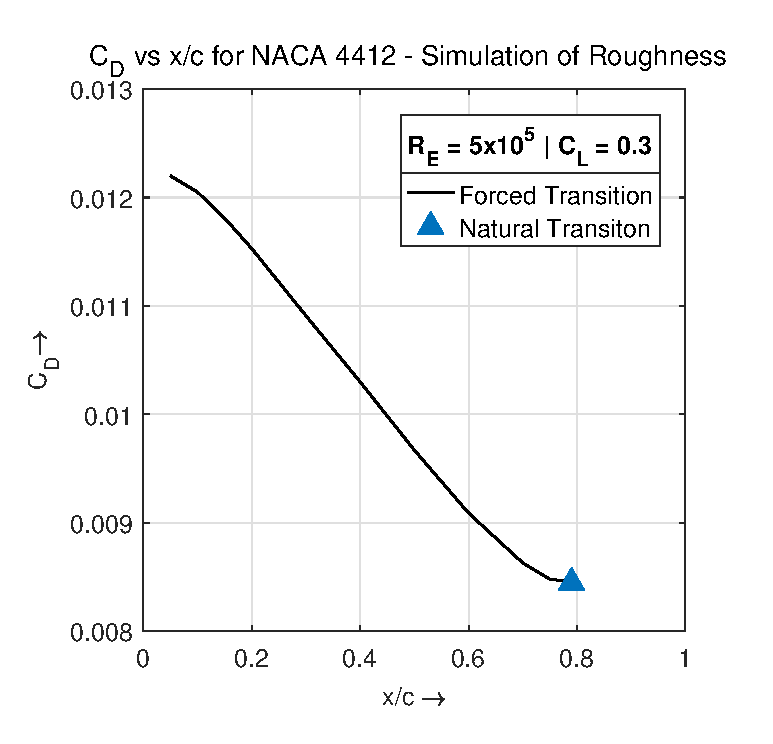
\includegraphics[width=0.5\textwidth]{./Images/Ass2/Cd_X_NACA4412_TRANSITION} 
\caption{$C_D$ vs $N_{crit}$ for NACA 4412}
\label{Fig5}
\end{figure}
\vspace*{-0.5em}

\printbibliography[title={References}]

\end{document}
